\documentclass[11pt,a4paper]{article}

% ------------------------------------------------------------------
%  Building Accessible Android Applications — Case Study: Podcast App
%  Group report (English). Compile with pdflatex (run twice for ToC).
% ------------------------------------------------------------------

% Compile with XeLaTeX (Unicode/Vietnamese names handled natively via fontspec).
\usepackage{fontspec}
\setmainfont{Libertinus Serif}
\setmonofont{Cascadia Code}[Scale=0.88]
\usepackage[a4paper,margin=2.4cm]{geometry}
\usepackage{graphicx}
\usepackage{xcolor}
\usepackage{booktabs}
\usepackage{tabularx}
\usepackage{array}
\usepackage{enumitem}
\usepackage{caption}
\usepackage{subcaption}
\usepackage{listings}
\usepackage{tikz}
\usetikzlibrary{arrows.meta,positioning,shapes.geometric,fit,backgrounds,calc}
\usepackage{fancyhdr}
\usepackage{titlesec}
\usepackage[hidelinks]{hyperref}

% ---- Palette (mirrors the app theme) -----------------------------
\definecolor{brandblue}{HTML}{3B5BDB}
\definecolor{brandgreen}{HTML}{12B886}
\definecolor{ink}{HTML}{1A1C1E}
\definecolor{slate}{HTML}{44474E}
\definecolor{softbg}{HTML}{F2F4F9}
\definecolor{codebg}{HTML}{F7F8FB}
\definecolor{codekw}{HTML}{2B6CB0}
\definecolor{codestr}{HTML}{2F9E44}
\definecolor{codecom}{HTML}{868E96}
\definecolor{codeann}{HTML}{9C36B5}
\definecolor{warnred}{HTML}{B02A37}

% ---- Section styling ---------------------------------------------
\titleformat{\section}{\Large\bfseries\color{brandblue}}{\thesection}{0.6em}{}
\titleformat{\subsection}{\large\bfseries\color{ink}}{\thesubsection}{0.6em}{}
\titleformat{\subsubsection}{\normalsize\bfseries\color{slate}}{\thesubsubsection}{0.6em}{}

\pagestyle{fancy}
\fancyhf{}
\fancyhead[L]{\small\itshape Building Accessible Android Applications}
\fancyhead[R]{\small Podcast Case Study}
\fancyfoot[C]{\thepage}
\renewcommand{\headrulewidth}{0.4pt}

\captionsetup{font=small,labelfont={bf,color=brandblue}}

% ---- Kotlin listing style ----------------------------------------
\lstdefinelanguage{Kotlin}{
  keywords={package,import,fun,val,var,class,object,interface,if,else,when,for,while,return,true,false,null,private,public,override,companion,by,this,is,as,in,data,sealed,enum,lateinit,remember,Composable},
  keywordstyle=\color{codekw}\bfseries,
  ndkeywords={Modifier,Text,Icon,IconButton,Box,Row,Column,Card,Scaffold,Role,Color,String,Boolean,Float,Unit,List,Int},
  ndkeywordstyle=\color{brandgreen}\bfseries,
  sensitive=true,
  comment=[l]{//},
  morecomment=[s]{/*}{*/},
  commentstyle=\color{codecom}\itshape,
  stringstyle=\color{codestr},
  morestring=[b]",
  morestring=[b]',
}
\lstdefinestyle{kt}{
  language=Kotlin,
  backgroundcolor=\color{codebg},
  basicstyle=\ttfamily\footnotesize,
  breaklines=true,
  breakatwhitespace=true,
  columns=fullflexible,
  keepspaces=true,
  showstringspaces=false,
  frame=leftline,
  framerule=2pt,
  rulecolor=\color{brandblue},
  xleftmargin=10pt,
  aboveskip=8pt,
  belowskip=8pt,
  moredelim=[il][\color{codeann}]{@},
}
\lstset{style=kt}

% ---- Helper commands ---------------------------------------------
\newcommand{\code}[1]{\colorbox{softbg}{\texttt{\small #1}}}
\newcolumntype{Y}{>{\raggedright\arraybackslash}X}

\setlength{\parskip}{0.5em}
\setlength{\parindent}{0pt}

\begin{document}

\begin{titlepage}
\centering
\vspace*{1.2cm}

{\Large\bfseries\color{brandblue} Building Accessible Android Applications\par}
\vspace{0.4cm}
{\large A Case Study on an Accessible Podcast \& Audiobook App\par}
{\large built with Jetpack Compose and Kotlin\par}

\vspace{1.0cm}

\begin{tikzpicture}
  \fill[brandblue,rounded corners=10pt] (0,0) rectangle (2.2,2.2);
  \node[white,font=\Huge\bfseries] at (1.1,1.35) {P};
  \fill[white] (0.75,0.35) rectangle (1.45,0.9);
  \fill[brandblue] (0.95,0.45) rectangle (1.05,0.8);
  \fill[brandblue] (1.15,0.45) rectangle (1.25,0.8);
\end{tikzpicture}

\vspace{1.0cm}
{\itshape A technical report on semantic accessibility, screen-reader support,\\ and accessibility testing in modern Android UI development.\par}

\vspace{1.4cm}
{\large\bfseries Group of 4\par}
\vspace{0.4cm}
{\normalsize Phát \quad$\bullet$\quad Phong \quad$\bullet$\quad Khương \quad$\bullet$\quad Tính\par}

\vfill
{\small Course: Mobile Application Development \quad$\bullet$\quad Group of 4\par}
{\small \today\par}
\end{titlepage}

\clearpage
\tableofcontents
\clearpage

\section{Introduction}

\subsection{Motivation}

Roughly one in six people worldwide lives with a significant disability. For many of them an
assistive device is the primary way for them to perceive and interact with the world.
Accessibility is the practice of designing hardware and software so that people with
temporary or permanent physical, sensory, or cognitive differences have an equal opportunity to use them. Unavailibility of accessible features exclude a portion of the population from conveniences of electronic, which we might argue that they are effectively isolated from communication. Building inclusively is therefore both an act of basic
fairness and, increasingly, a legal obligation.

This report documents our group research on existing norms and regulation around the inclusiveness that applications should implements, as well as how our group apply them to a podcast and audiobook player to be usable by people who rely on assistive technology such as the TalkBack screen reader, Switch Access, and large display fonts. We chose an
audio-first product as listening to audio content is one of the few digital experiences that a user with vision problems can enjoy on completely equal terms with a normal vision user,

\subsection{Project goal and scope}

Our goal was to take a typical, non-inclusive to vision-impaired people UI and improve it into an accessible one, then explain and justify every technique we applied. The deliverable is a front-end only Jetpack Compose application (all data is mocked behind a repository interface, with no real backend) along with this report, which is organised around four contributions:

\begin{itemize}[leftmargin=1.4em]
	\item \textbf{Background} : the legal and technical foundations of Android accessibility.
	\item \textbf{Core semantics} : labelling, roles, state, touch targets, and font scaling.
	\item \textbf{Advanced semantics} : merging, traversal order, and custom screen-reader actions.
	\item \textbf{Testing and evaluation} : how we verify the result and honestly assess trade-offs.
\end{itemize}

\subsection{What ``done'' looks like}

Throughout the project we held ourselves to a simple bar: a person who never looks at the
screen should be able to open the app, browse shows, pick an episode, and control playback using
TalkBack alone. Figure~\ref{fig:appflow} shows the three-screen user flow that a sighted user sees;
the rest of the report explains what a screen-reader user hears and does at each step.

\begin{figure}[h]
	\centering
	\begin{subfigure}{0.31\textwidth}
		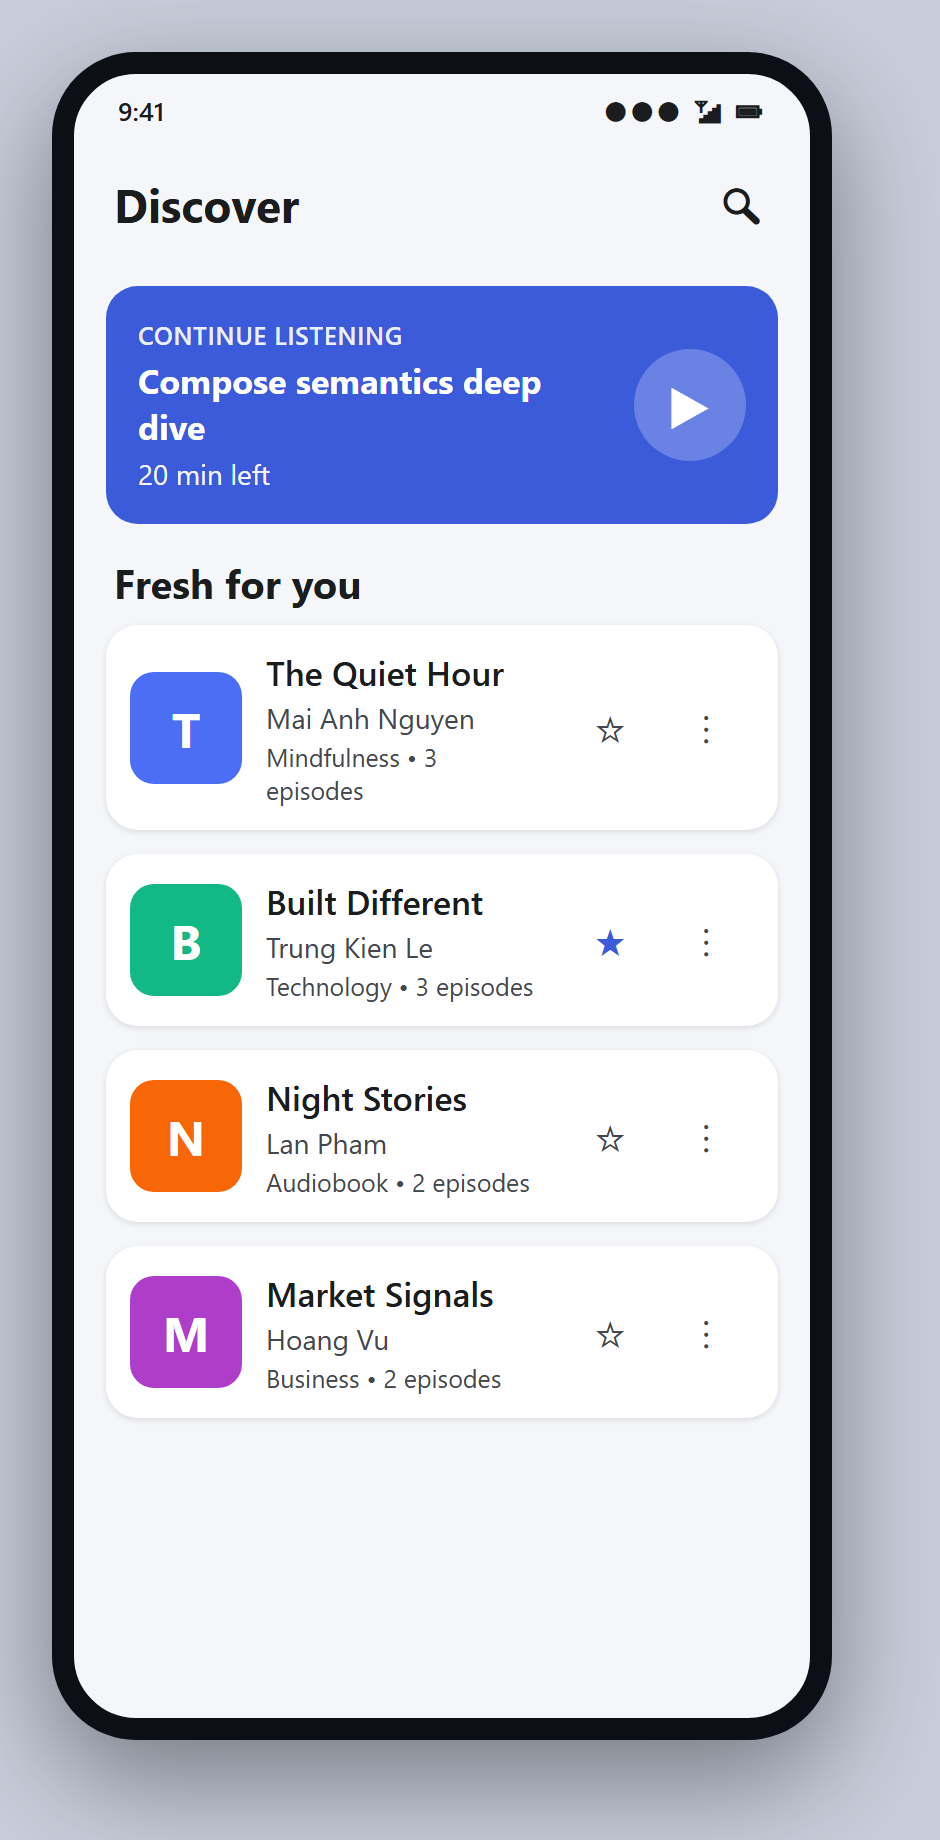
\includegraphics[width=\linewidth]{images/home.png}
		\caption{Discover}
	\end{subfigure}\hfill
	\begin{subfigure}{0.31\textwidth}
		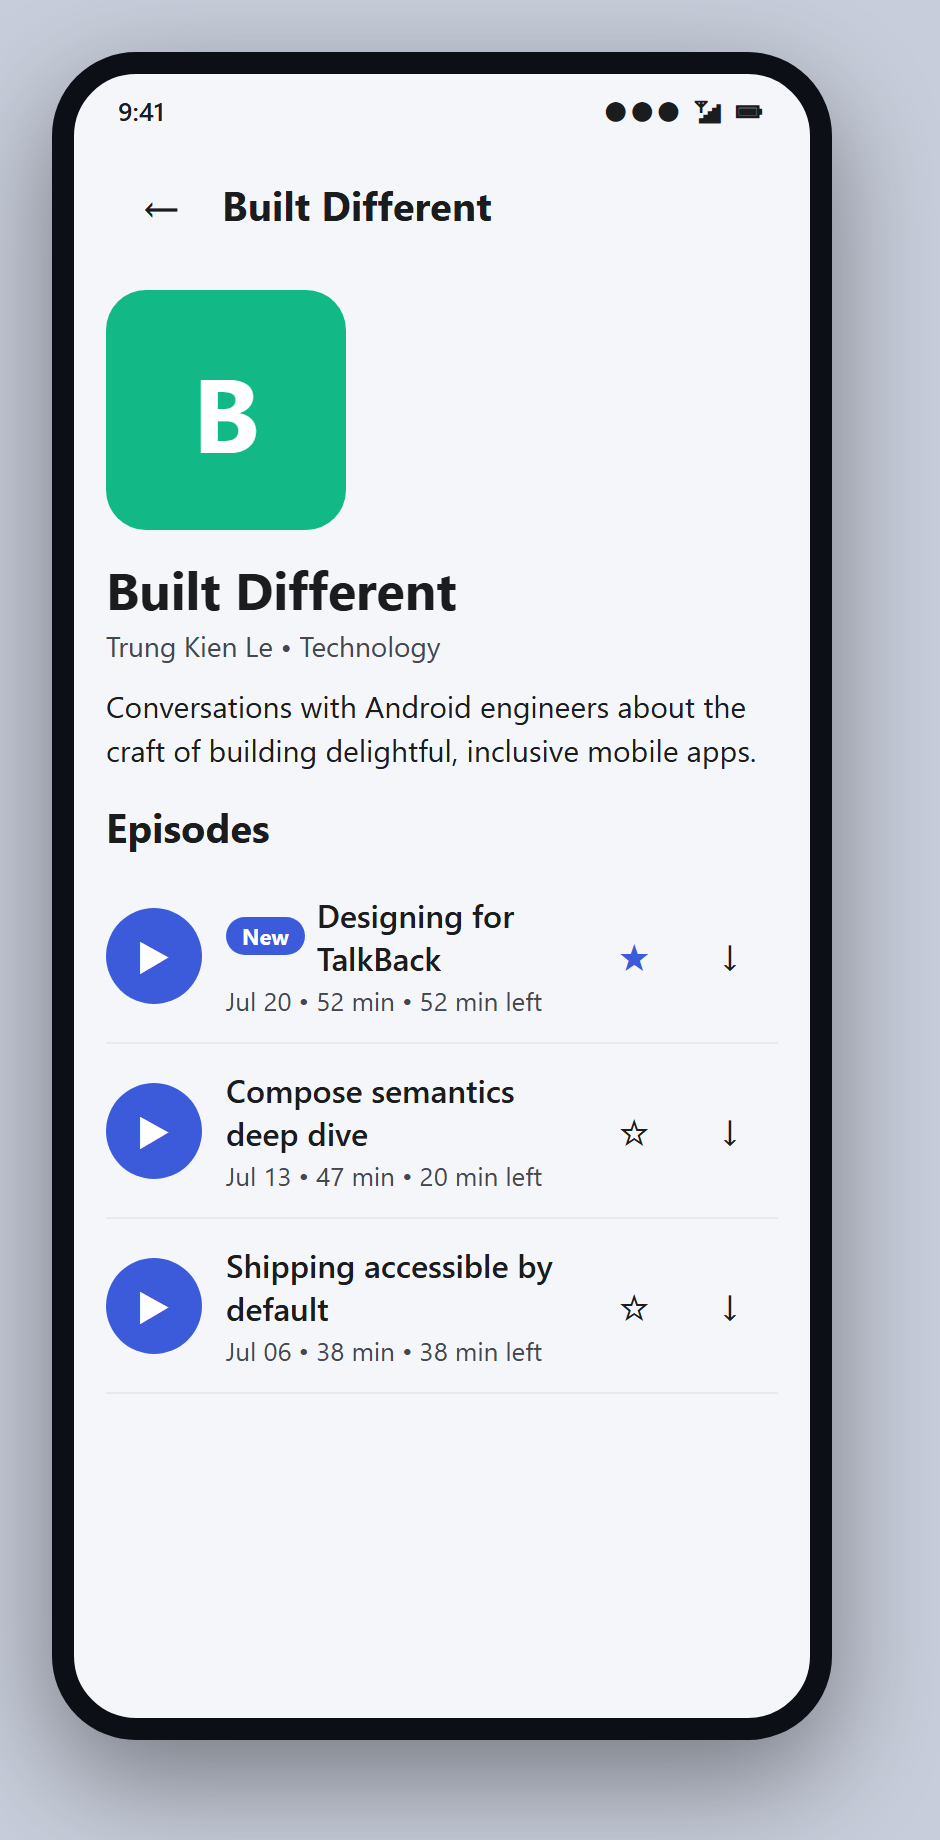
\includegraphics[width=\linewidth]{images/detail.png}
		\caption{Podcast detail}
	\end{subfigure}\hfill
	\begin{subfigure}{0.31\textwidth}
		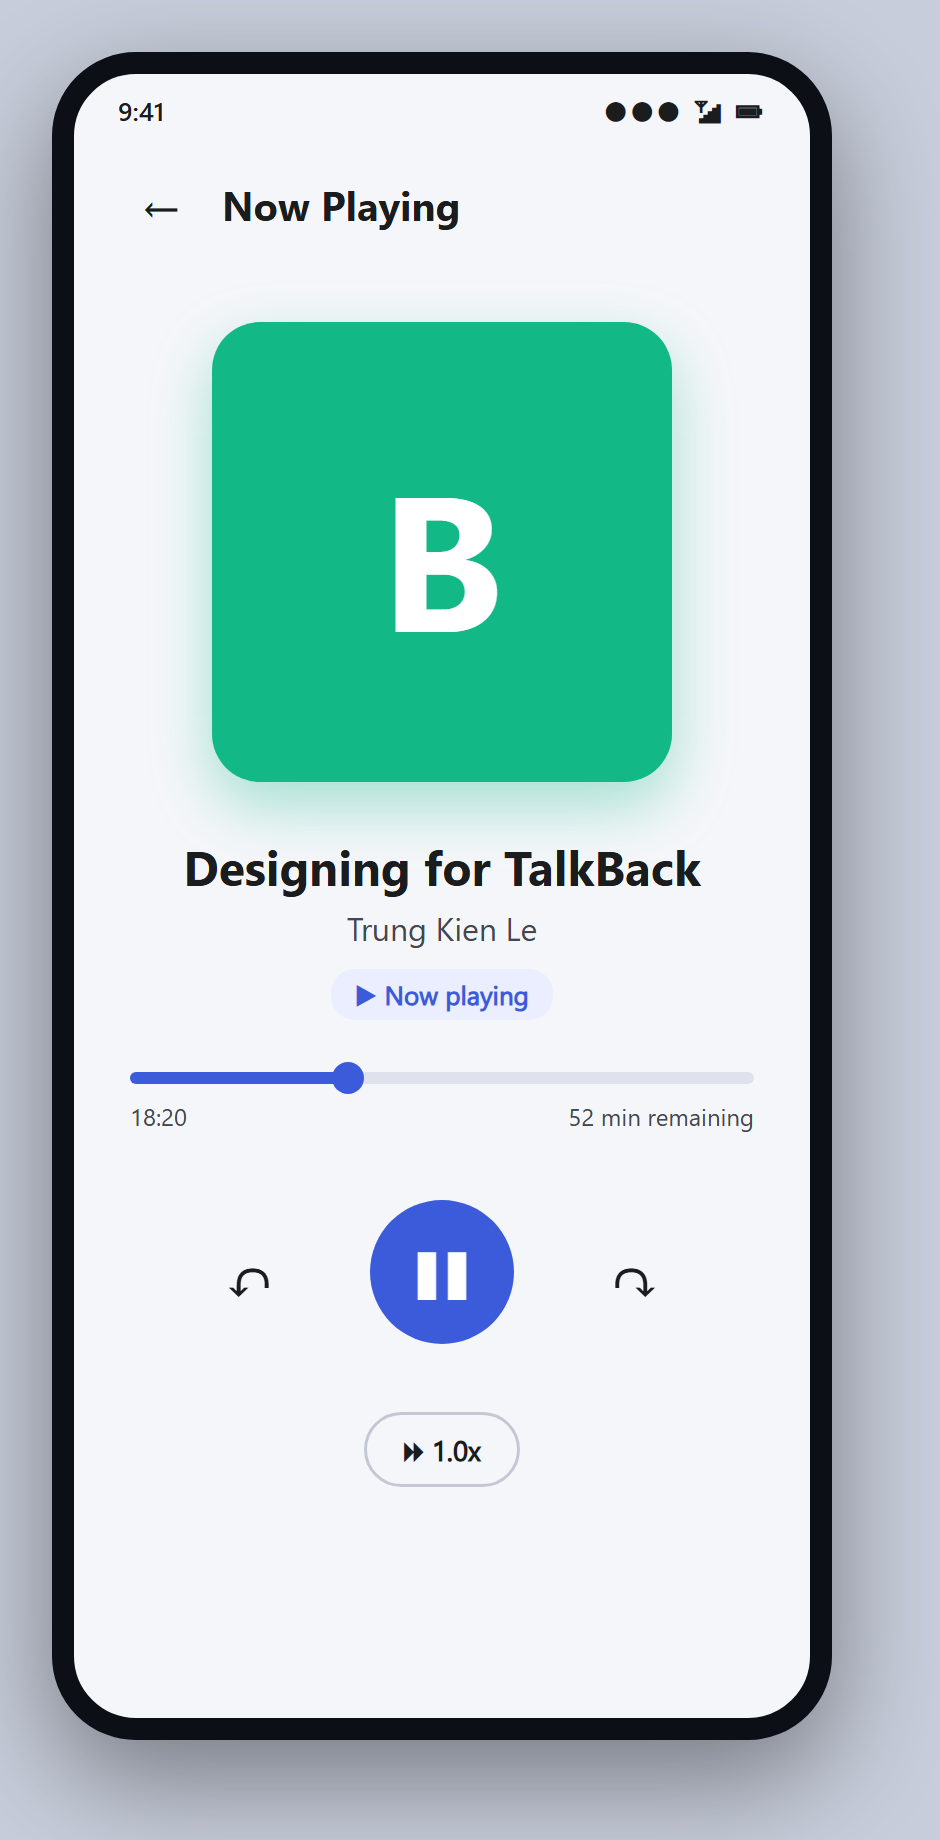
\includegraphics[width=\linewidth]{images/player.png}
		\caption{Now Playing}
	\end{subfigure}
	\caption{The three screens of the case-study app. The user flow is
		\textbf{Discover $\rightarrow$ Podcast detail $\rightarrow$ Now Playing}, with a
		``Continue listening'' shortcut on the home screen.}
	\label{fig:appflow}
\end{figure}

\section{Background}
\label{sec:bg}

\subsection{The legal driver}
\label{sec:legal}

The \textbf{European Accessibility Act} (Directive (EU) 2019/882) requires products sold in the EU to
meet common accessibility requirements; every member state transposed it into national law by
June~2022. Its technical yardstick is \textbf{WCAG~2.2}. WCAG targets the web, so for a native app we
apply it through \emph{WCAG2ICT} and mobile guidance --- mapping each success criterion to its
Android equivalent rather than claiming literal conformance.

\subsection{The POUR principles}

WCAG rests on four principles (Figure~\ref{fig:pour}). For a media player they read concretely as:

\begin{itemize}[leftmargin=1.4em,itemsep=1pt]
	\item \textbf{Perceivable} --- label every transport icon; keep duration text at $\geq$4.5:1 contrast.
	\item \textbf{Operable} --- play, seek, and bookmark reachable from TalkBack, not only by touch.
	\item \textbf{Understandable} --- the play button announces ``playing'' vs.\ ``paused''.
	\item \textbf{Robust} --- expose a correct semantics tree instead of relying on pixels.
\end{itemize}

\begin{figure}[h]
	\centering
	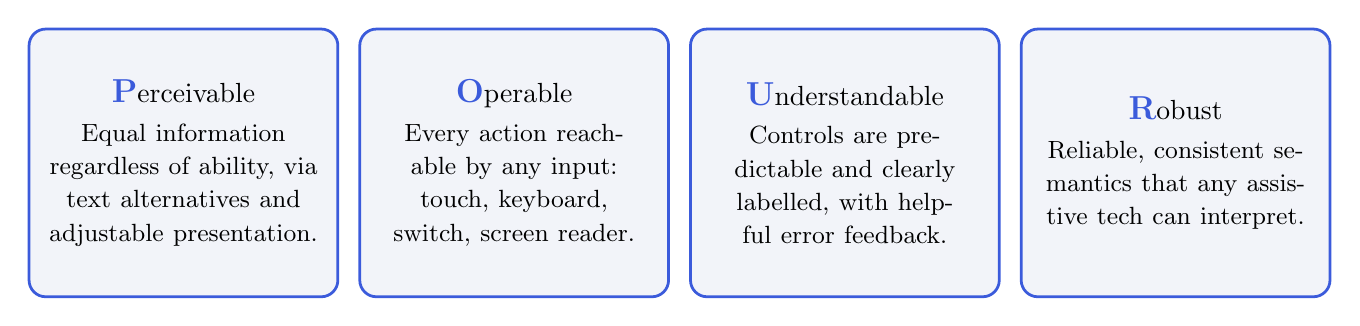
\begin{tikzpicture}[
			box/.style={rounded corners=6pt,draw=brandblue,line width=1pt,fill=softbg,
					text width=3.5cm,minimum height=3.4cm,align=center,inner sep=6pt},
		]
		\def\cap#1{{\large\bfseries\color{brandblue}#1}}
		\node[box] (p) at (0,0) {\cap{P}erceivable\\[2pt]\small Equal information regardless of ability, via text alternatives and adjustable presentation.};
		\node[box] (o) at (4.2,0) {\cap{O}perable\\[2pt]\small Every action reachable by any input: touch, keyboard, switch, screen reader.};
		\node[box] (u) at (8.4,0) {\cap{U}nderstandable\\[2pt]\small Controls are predictable and clearly labelled, with helpful error feedback.};
		\node[box] (r) at (12.6,0) {\cap{R}obust\\[2pt]\small Reliable, consistent semantics that any assistive tech can interpret.};
	\end{tikzpicture}
	\caption{The four POUR principles that underpin WCAG.}
	\label{fig:pour}
\end{figure}

\subsection{Two trees, one screen}

The decisive fact for an Android developer: what is drawn and what a screen reader traverses are
\emph{two separate trees} (Figure~\ref{fig:trees}).

\begin{itemize}[leftmargin=1.4em,itemsep=1pt]
	\item \textbf{Composition tree} --- the visual hierarchy; nodes are boxes, text, and images ordered
	      by draw position.
	\item \textbf{Semantics tree} --- runs in parallel; each node carries a name, role, state, and
	      supported actions. It is the only thing assistive services can read.
\end{itemize}

\begin{figure}[h]
	\centering
	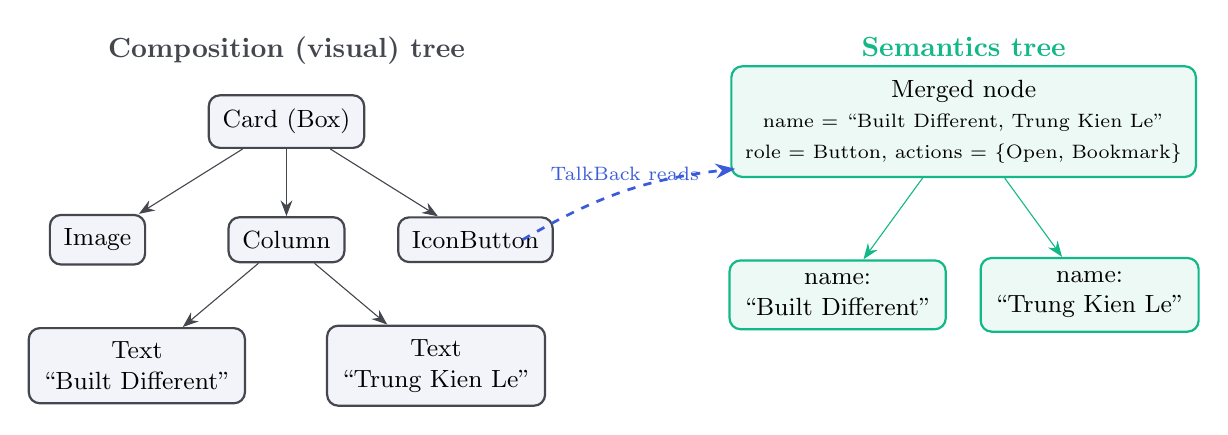
\begin{tikzpicture}[
		n/.style={rounded corners=4pt,draw,line width=0.8pt,font=\small,inner sep=5pt,align=center},
		vis/.style={n,draw=slate,fill=softbg},
		sem/.style={n,draw=brandgreen,fill=brandgreen!8},
		e/.style={-{Stealth[length=2mm]},draw=slate},
		se/.style={-{Stealth[length=2mm]},draw=brandgreen}
		]
		% Visual tree
		\node[vis] (root) at (0,0) {Card (Box)};
		\node[vis] (img)  at (-2.4,-1.5) {Image};
		\node[vis] (col)  at (0,-1.5) {Column};
		\node[vis] (btn)  at (2.4,-1.5) {IconButton};
		\node[vis] (t1)   at (-1.9,-3.1) {Text\\``Built Different''};
		\node[vis] (t2)   at (1.9,-3.1) {Text\\``Trung Kien Le''};
		\draw[e] (root)--(img); \draw[e] (root)--(col); \draw[e] (root)--(btn);
		\draw[e] (col)--(t1); \draw[e] (col)--(t2);
		\node[font=\bfseries\color{slate}] at (0,0.9) {Composition (visual) tree};

		% Semantics tree
		\begin{scope}[xshift=8.6cm]
			\node[sem] (sroot) at (0,0) {Merged node\\{\scriptsize name = ``Built Different, Trung Kien Le''}\\{\scriptsize role = Button, actions = \{Open, Bookmark\}}};
			\node[sem] (s1) at (-1.6,-2.2) {name:\\``Built Different''};
			\node[sem] (s2) at (1.6,-2.2) {name:\\``Trung Kien Le''};
			\draw[se] (sroot)--(s1); \draw[se] (sroot)--(s2);
			\node[font=\bfseries\color{brandgreen}] at (0,0.95) {Semantics tree};
		\end{scope}

		\draw[-{Stealth[length=2.5mm]},brandblue,line width=1pt,dashed]
		(3.0,-1.5) to[bend left=12] node[above,font=\scriptsize\color{brandblue}]{TalkBack reads} (5.7,-0.6);
	\end{tikzpicture}
	\caption{The visual tree (left) is drawn; the semantics tree (right) is read by TalkBack. The
		decorative image is dropped and the two texts are \emph{merged} into one node --- the techniques
		of §\ref{sec:core} and~§\ref{sec:adv}.}
	\label{fig:trees}
\end{figure}

TalkBack and Switch Access run as system services that subscribe to the \emph{merged} semantics tree,
turn each node into speech or a scan stop, and translate gestures back into actions. A pixel-perfect
screen is unusable if its semantics tree is missing, mislabelled, or misordered. Every technique in
this report shapes that tree.

\subsection{Jetpack Compose}

Compose is Android's declarative UI toolkit: the UI is a function of state, and state changes trigger
recomposition. It builds the semantics tree from Material components' built-in semantics plus
\code{Modifier.semantics} blocks --- giving code-level control over exactly what assistive technology
perceives.

\section{The Case-Study App: Accessible Podcast}
\label{sec:casestudy}

\subsection{Overview}

We built \textbf{Accessible Podcast}, a complete front-end Compose app, to ground the techniques. An
in-memory mock implements the \code{PodcastRepository} interface, so the UI code is identical to a real-backend version but runs anywhere with no configuration.

\subsection{User flow}

The app implements the classic three-step listening flow, plus a resume shortcut
(Figure~\ref{fig:flow}).

\begin{figure}[h]
	\centering
	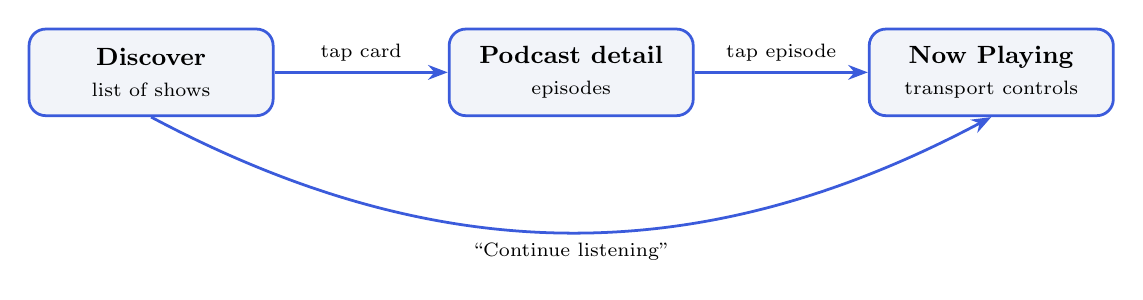
\begin{tikzpicture}[
		s/.style={rounded corners=6pt,draw=brandblue,line width=1pt,fill=softbg,
				minimum width=3.1cm,minimum height=1.1cm,align=center,font=\small},
		a/.style={-{Stealth[length=2.5mm]},draw=brandblue,line width=1pt,font=\scriptsize}
		]
		\node[s] (h) {\textbf{Discover}\\{\scriptsize list of shows}};
		\node[s,right=2.2cm of h] (d) {\textbf{Podcast detail}\\{\scriptsize episodes}};
		\node[s,right=2.2cm of d] (p) {\textbf{Now Playing}\\{\scriptsize transport controls}};
		\draw[a] (h) -- node[above]{tap card} (d);
		\draw[a] (d) -- node[above]{tap episode} (p);
		\draw[a] (h.south) to[bend right=28] node[below,pos=0.5]{``Continue listening''} (p.south);
	\end{tikzpicture}
	\caption{User flow. Each transition is reachable by TalkBack double-tap and by Switch Access.}
	\label{fig:flow}
\end{figure}

\subsection{Architecture}

The code is organised into a thin data layer and a Compose UI layer
(Figure~\ref{fig:arch}). The UI depends
only on the \code{PodcastRepository} interface, never on the mock, thus we can substitute a real backend in without changing the UI's declaration and logic.

\begin{figure}[h]
	\centering
	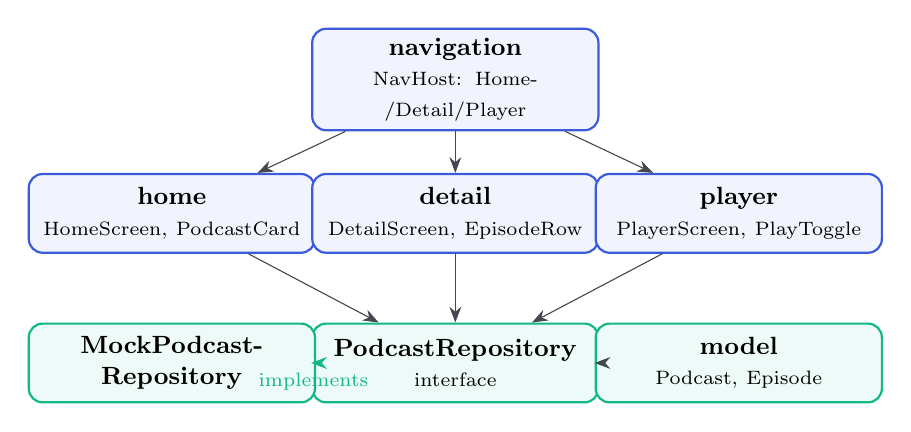
\begin{tikzpicture}[
		layer/.style={rounded corners=5pt,draw,line width=0.8pt,minimum height=1cm,align=center,font=\small,text width=3.4cm},
		ui/.style={layer,draw=brandblue,fill=brandblue!7},
		dm/.style={layer,draw=brandgreen,fill=brandgreen!7},
		e/.style={-{Stealth[length=2mm]},draw=slate}
		]
		\node[ui] (nav) at (0,0) {\textbf{navigation}\\{\scriptsize NavHost: Home/Detail/Player}};
		\node[ui] (home) at (-3.6,-1.7) {\textbf{home}\\{\scriptsize HomeScreen, PodcastCard}};
		\node[ui] (det) at (0,-1.7) {\textbf{detail}\\{\scriptsize DetailScreen, EpisodeRow}};
		\node[ui] (play) at (3.6,-1.7) {\textbf{player}\\{\scriptsize PlayerScreen, PlayToggle}};
		\node[dm] (repo) at (0,-3.6) {\textbf{PodcastRepository}\\{\scriptsize interface}};
		\node[dm] (mock) at (-3.6,-3.6) {\textbf{MockPodcast\-Repository}};
		\node[dm] (model) at (3.6,-3.6) {\textbf{model}\\{\scriptsize Podcast, Episode}};
		\draw[e] (nav)--(home); \draw[e] (nav)--(det); \draw[e] (nav)--(play);
		\draw[e] (home)--(repo); \draw[e] (det)--(repo); \draw[e] (play)--(repo);
		\draw[e,dashed,brandgreen] (mock)-- node[below,font=\scriptsize]{implements} (repo);
		\draw[e] (repo)--(model);
	\end{tikzpicture}
	\caption{Package architecture. The Compose UI layer (blue) talks to a single repository interface;
		the mock (green) is the only implementation and can be swapped for a real one with no UI change.}
	\label{fig:arch}
\end{figure}

\subsection{The mock data layer}

The repository exposes an observable catalogue as a \code{StateFlow}. Toggling a bookmark mutates the
flow, so every screen recomposes exactly as it would against a reactive backend, which also lets
us verify that state changes are announced to TalkBack.

\begin{lstlisting}[caption={The repository interface the whole UI depends on.},captionpos=b]
interface PodcastRepository {
    val podcasts: StateFlow<List<Podcast>>   // observable catalogue
    fun getEpisode(id: String): Episode?
    fun toggleBookmark(episodeId: String)     // mutates state -> recomposition
    fun toggleDownload(episodeId: String)
}
\end{lstlisting}

\subsection{Where each technique lives}

Table~\ref{tab:map} maps every accessibility technique discussed in this report to the exact file in
the project, so the demo and the prose stay in lock-step.

\begin{table}[h]
	\centering
	\small
	\begin{tabularx}{\textwidth}{@{}l l Y@{}}
		\toprule
		\textbf{Report section}   & \textbf{Technique}                                 & \textbf{File}                                   \\
		\midrule
		Core (§\ref{sec:core})    & \code{contentDescription}, decorative \code{null}  & \texttt{ui/components/CoverArt.kt}              \\
		Core                      & \code{Role.Button} + \code{stateDescription}       & \texttt{ui/player/PlayToggle.kt}                \\
		Core                      & 48\,dp touch targets                               & \texttt{ui/home/PodcastCard.kt}                 \\
		Core                      & \code{sp} typography, font scaling                 & \texttt{ui/theme/Type.kt}                       \\
		Core                      & heading navigation                                 & \texttt{ui/home/HomeScreen.kt}                  \\
		Advanced (§\ref{sec:adv}) & \code{mergeDescendants}                            & \texttt{PodcastCard.kt}, \texttt{EpisodeRow.kt} \\
		Advanced                  & \code{clearAndSetSemantics} + \code{customActions} & \texttt{EpisodeRow.kt}                          \\
		Advanced                  & \code{hideFromAccessibility}                       & \texttt{CoverArt.kt}                            \\
		Advanced                  & \code{isTraversalGroup} + \code{traversalIndex}    & \texttt{HomeScreen.kt}                          \\
		Background                & \code{liveRegion} announcements                    & \texttt{ui/player/PlayerScreen.kt}              \\
		Testing (§\ref{sec:test}) & Compose assertions, ATF                            & \texttt{androidTest/AccessibilityTest.kt}       \\
		\bottomrule
	\end{tabularx}
	\caption{Technique-to-file map. Every claim in the report is backed by runnable code.}
	\label{tab:map}
\end{table}

\section{Technical Approach I --- Core Semantics}
\label{sec:core}

Five modifiers make a single component accessible --- labelling, roles, state, touch-target size, and
scalable type. They fix the most common and most damaging screen-reader defects.

\subsection{Content descriptions: naming visual elements}

A screen reader cannot see an icon; it can only read the icon's text alternative --- in Compose, the
\code{contentDescription} parameter. Three rules make a good label:

\begin{itemize}[leftmargin=1.4em]
	\item \textbf{Succinct \& action-oriented.} Avoid ``Image of'' / ``Button to''. The element's name is
	      announced separately.
	\item \textbf{Localized.} Always use \code{stringResource()} so labels translate with the device
	      language.
	\item \textbf{Hide the decorative.} Purely decorative graphics must be removed from the tree so
	      they do not add noise.
\end{itemize}

\begin{lstlisting}[caption={Meaningful icons get a localized label; decorative art is hidden.},captionpos=b]
// Meaningful control — announced as "Search podcasts, button"
Icon(
    imageVector = Icons.Filled.Search,
    contentDescription = stringResource(R.string.cd_search)
)

// Decorative cover tile — next to a text title, so it adds nothing for TalkBack
Box(
    modifier = Modifier.size(56.dp).background(color)
        .semantics { hideFromAccessibility() }   // Compose 1.8+; still visible to UI tests
)
\end{lstlisting}

In practice: Instagram labels its action buttons (``Like'', ``Comment'') but passes \code{null} to
the decorative story gradients, so screen-reader users jump straight between real content.

\subsection{Roles and state descriptions on custom controls}

Material components carry their own semantics, but a custom control built from a bare \code{Box} tells
assistive tech nothing. We must declare two things explicitly: a \textbf{role} (so TalkBack appends
``Button''/``Switch'') and, for anything toggleable, a \textbf{state description} (the dynamic
``Playing''/``Paused''). Our circular player button, taken directly from the app, does both:

\begin{lstlisting}[caption={\texttt{PlayToggle.kt} --- a custom control with an explicit role and a dynamic state.},captionpos=b]
@Composable
fun PlayToggle(isPlaying: Boolean, onToggle: () -> Unit) {
    val name = stringResource(if (isPlaying) R.string.cd_pause else R.string.cd_play)
    val state = stringResource(if (isPlaying) R.string.state_playing else R.string.state_paused)
    Box(
        modifier = Modifier.size(72.dp).clip(CircleShape).background(primary)
            .clickable(onClick = onToggle, role = Role.Button)
            .semantics {
                contentDescription = name       // "Play" / "Pause"
                stateDescription = state         // "Playing" / "Paused"
                role = Role.Button
            },
        contentAlignment = Alignment.Center
    ) {
        Icon(imageVector = icon, contentDescription = null) // handled by the Box
    }
}
\end{lstlisting}

TalkBack now announces \emph{``Pause, button, Playing''} --- name, role, and state --- which is
exactly how Spotify's custom playback control behaves.

\subsection{Touch-target sizing}

Users with motor impairments, or anyone tapping on a moving bus, need a target they can hit
reliably. Material Design mandates a minimum interactive size of \textbf{48\,dp $\times$ 48\,dp}
(WCAG~2.5.5 asks for 44\,px). The visual icon can stay small; only the \emph{touchable area} must
grow. Compose does this automatically for Material components and, for custom ones, via
\code{minimumInteractiveComponentSize()}:

\begin{lstlisting}[caption={A 24\,dp icon with a guaranteed 48\,dp touch target.},captionpos=b]
IconButton(
    onClick = onToggleBookmark,
    modifier = Modifier
        .minimumInteractiveComponentSize()   // expands hit area to 48dp, no visual change
        .clearAndSetSemantics {}             // (see advanced section)
) { Icon(Icons.Filled.BookmarkBorder, contentDescription = null) }
\end{lstlisting}

This is the same pattern Gmail uses for the small ``star'' icon: a 24\,dp glyph with a 48\,dp hit
area, so users do not open the email by accident when they meant to star it.

\subsection{Scalable typography}

Android~14 introduced \textbf{non-linear font scaling} up to 200\%: small text grows a lot while
already-large headings grow less, preserving hierarchy. To benefit, code must separate \emph{text
	size} from \emph{layout size}:

\begin{enumerate}[leftmargin=1.4em]
	\item Text sizes always in \code{sp} --- Compose applies the non-linear math automatically.
	\item Paddings and constraints always in \code{dp}.
	\item \textbf{Never} hard-code a \code{height()} on a text container; use \code{defaultMinSize} or
	      padding so it can grow.
\end{enumerate}

Figure~\ref{fig:fontscale} shows why the third rule matters: a fixed-height card clips its text at
200\%, while the \code{sp}-based card grows gracefully. Our \code{Type.kt} defines every style in
\code{sp}, so the app passes this test out of the box.

\begin{figure}[h]
	\centering
	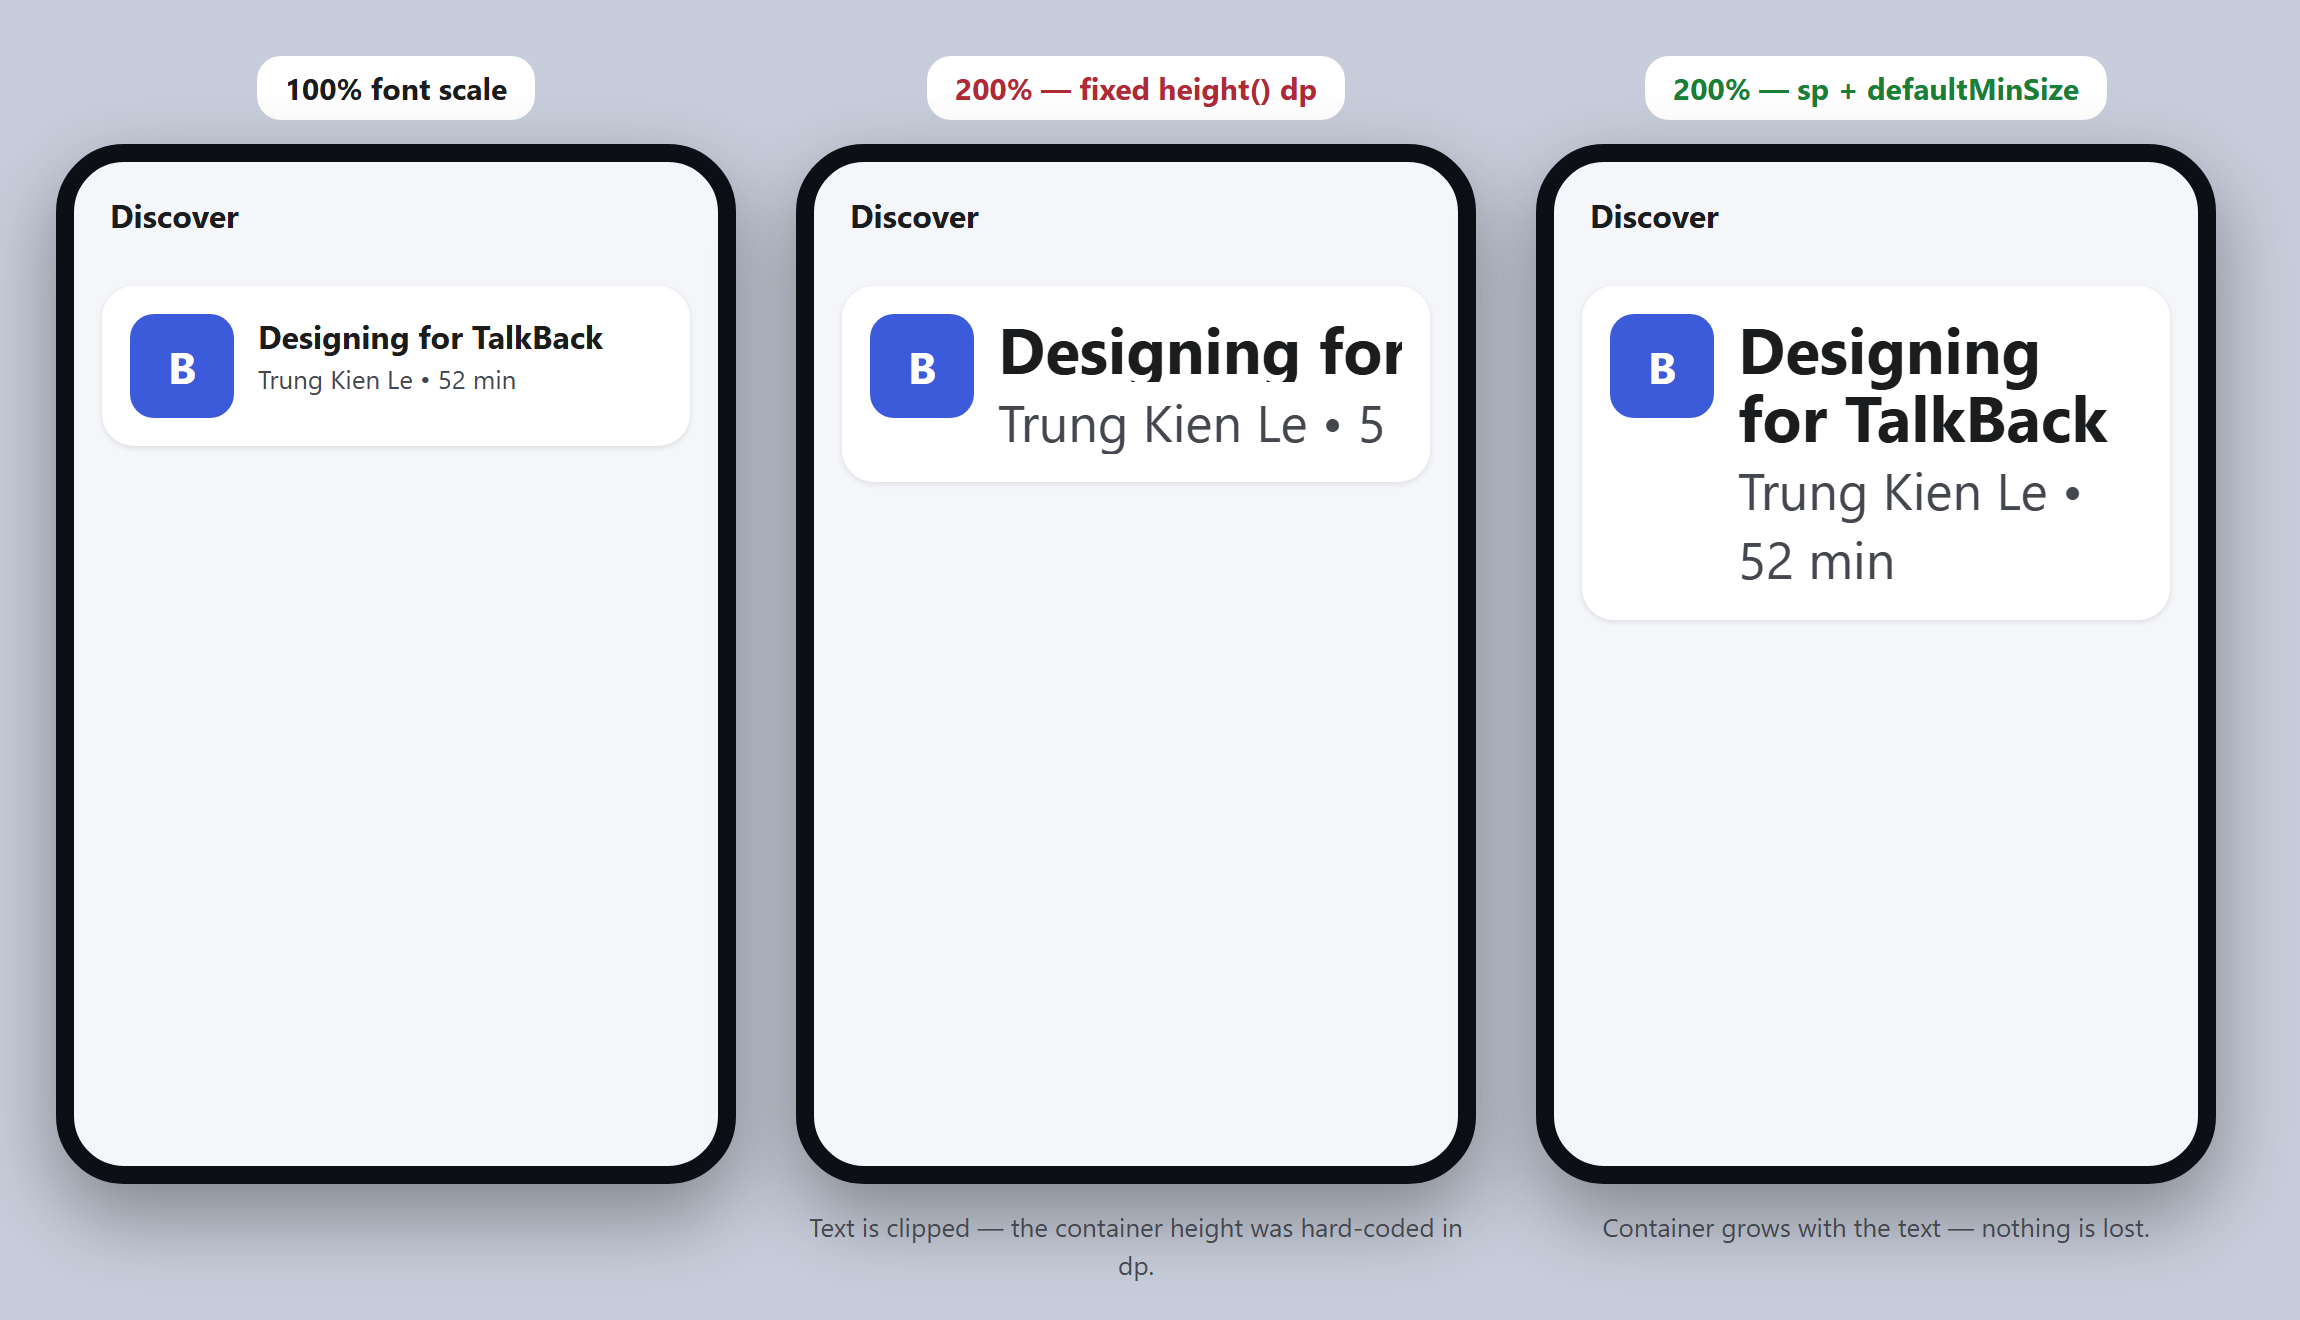
\includegraphics[width=\textwidth]{images/fontscale.png}
	\caption{The same card at 100\% and at 200\% font scale. A hard-coded \code{height()} in dp (centre)
		clips the title; \code{sp} text with \code{defaultMinSize} (right) lets the container expand so
		nothing is lost.}
	\label{fig:fontscale}
\end{figure}

\subsection{Heading navigation}

Finally, marking section titles with \code{semantics \{ heading() \}} lets TalkBack users jump
heading-to-heading instead of swiping through every item --- the screen-reader equivalent of
skimming. We apply it to the app-bar titles and the ``Fresh for you'' / ``Episodes'' headers.

\section{Technical Approach II --- Advanced Semantics \& Navigation}
\label{sec:adv}

Core semantics make one component correct; advanced semantics make a whole screen efficient to
navigate. They control how many focus stops exist, the order they are read in, and how nested actions
are reached, which create the difference between a automatically labelled UI and one that is fast to drive by
swipe or switch.

\subsection{Semantic merging}

By default every text node is its own focus stop. A podcast card with a cover, title, author, and
metadata therefore costs a TalkBack user 4--6 swipes to cross --- multiplied across a list of shows,
this is exhausting. \code{Modifier.semantics(mergeDescendants = true)} collapses a container's
children into one node whose announcement is the concatenation of its parts.

\begin{figure}[h]
	\centering
	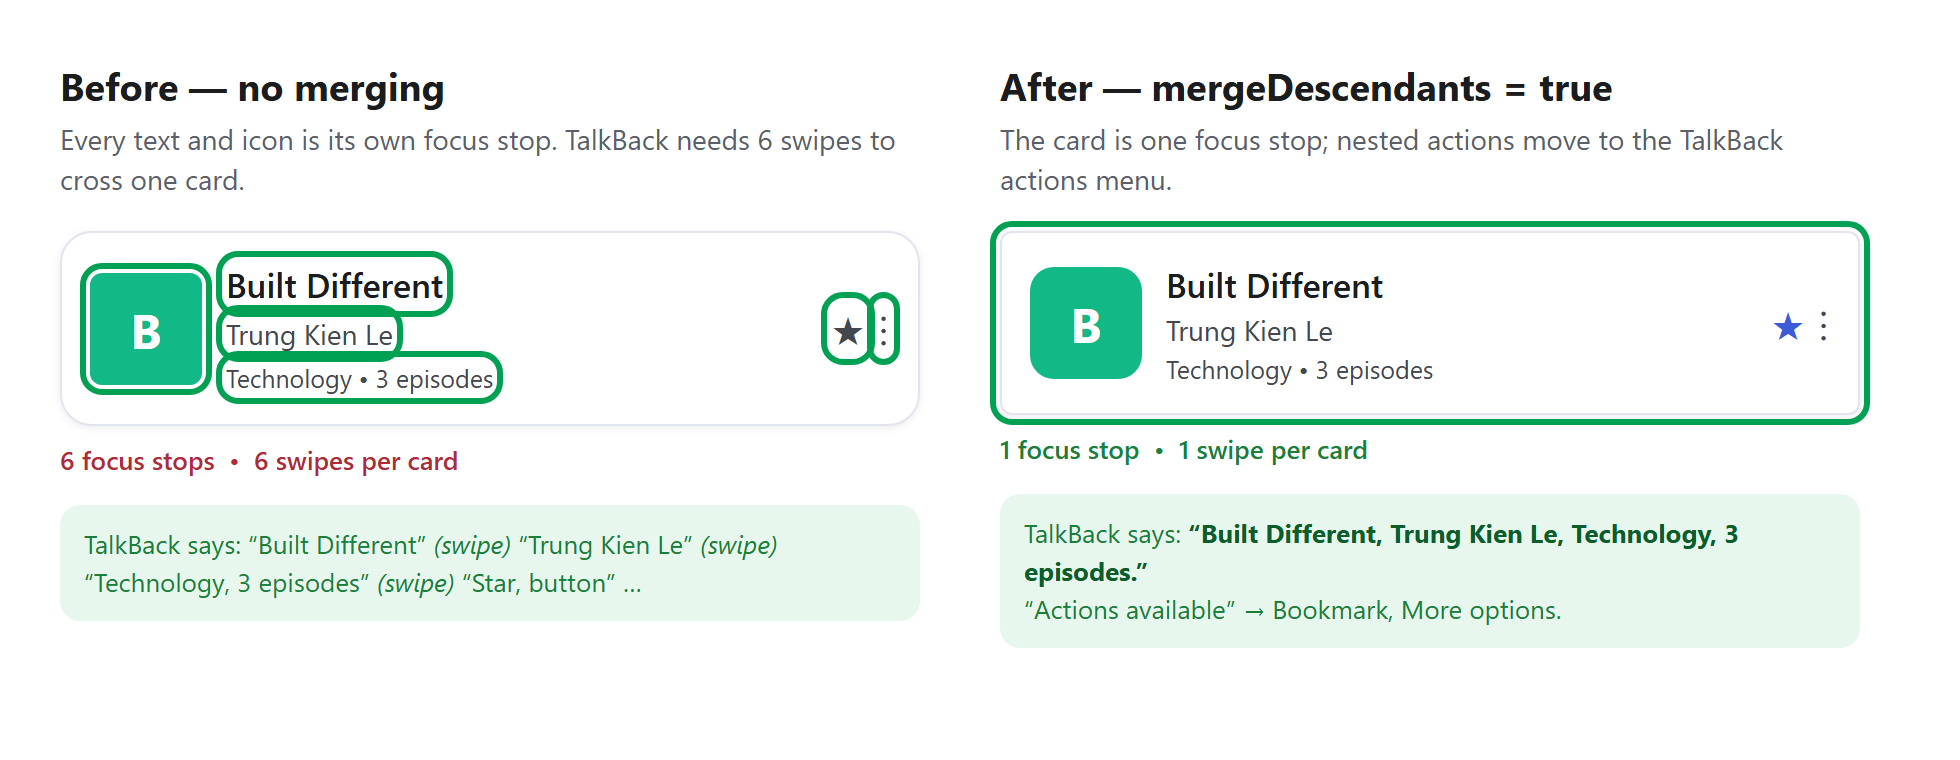
\includegraphics[width=\textwidth]{images/merge.png}
	\caption{The effect of \code{mergeDescendants = true} on a podcast card. Before (left): six separate
		focus stops, six swipes. After (right): one focus stop that TalkBack reads as a single sentence, with
		the nested bookmark/menu actions moved into the actions menu.}
	\label{fig:merge}
\end{figure}

\begin{lstlisting}[caption={\texttt{PodcastCard.kt} --- the card is one focus stop.},captionpos=b]
Card(
    onClick = onOpen,
    modifier = Modifier.semantics(mergeDescendants = true) {
        customActions = listOf(
            CustomAccessibilityAction(bookmarkLabel) { onToggleBookmark(latest); true }
        )
    }
) { /* cover + title + author + metadata + nested icon buttons */ }
\end{lstlisting}

There is a constraint on merging that a parent cannot merge a child that already merges itself. Interactive
components (\code{Button}, \code{Switch}, anything with \code{clickable}/\code{toggleable} modifiers) resist
merging so they remain independently operable. This is why the nested bookmark button needs
the next technique.

\subsection{Clearing and hiding with \texttt{clearAndSetSemantics} \& \texttt{hideFromAccessibility}}

Two modifiers prune the tree:

\begin{itemize}[leftmargin=1.4em]
	\item \code{clearAndSetSemantics \{\}} wipes a node's semantics (and its descendants') and lets us
	      redefine them  or leave them empty to remove the node from traversal entirely.
	\item \code{hideFromAccessibility()} (Compose~1.8+) hides a node from assistive services while
	      keeping it for UI tests. This is the modern alternative to setting
	      \code{contentDescription} to \code{null} on decorative elements.
\end{itemize}

In \code{CoverArt.kt} the coloured cover tile is decorative when a text title sits beside it, so we
hide it. In \code{EpisodeRow.kt} the three trailing icon buttons are cleared so they do not each
steal focus their actions are re-exposed on the row (next subsection).

\subsection{Custom accessibility actions}

Nested icon buttons are an anti-pattern for screen readers: they are tiny targets and they clutter
the swipe path (50 cards $\times$ 3 buttons = 150 extra swipes). The fix is to clear the
physical buttons and elevate their operations to \code{customActions} on the parent row, where
TalkBack surfaces them through its actions menu (``Actions available'').

\begin{lstlisting}[caption={\texttt{EpisodeRow.kt} --- nested actions promoted to the row's actions menu.},captionpos=b]
Row(
    modifier = Modifier.semantics(mergeDescendants = true) {
        customActions = listOf(
            CustomAccessibilityAction(playLabel)     { onPlay(); true },
            CustomAccessibilityAction(bookmarkLabel) { onToggleBookmark(); true },
            CustomAccessibilityAction(downloadLabel) { onToggleDownload(); true },
        )
    }
) {
    FilledIconButton(onClick = onPlay,
        modifier = Modifier.size(48.dp).clearAndSetSemantics {}) { /* icon */ }
    // ... title + metadata ...
    IconButton(onClick = onToggleBookmark,
        modifier = Modifier.minimumInteractiveComponentSize().clearAndSetSemantics {}) { /* icon */ }
}
\end{lstlisting}

A screen-reader user now hears the episode as one sentence, then opens ``Actions'' to Play, Bookmark,
or Download, while sighted users still tap the visible 48\,dp buttons directly.

\subsection{Traversal order}

Assistive tech normally reads in fixed order (top-to-bottom, then left-to-right), which breaks on non-linear
layouts. Two modifiers fix it: \code{isTraversalGroup = true} draws a boundary that must be read
completely before moving on, and \code{traversalIndex} (a \code{Float}, lowest first) reorders within
that boundary. A common pitfall is setting \code{traversalIndex} \emph{without} a group: because all
nodes default to \code{0f} globally, the element is compared against the whole screen and jumps to the
bottom. On the Discover screen we make the ``Continue listening'' banner read \emph{first} even though
it is not the top-most focusable item:

\begin{lstlisting}[caption={\texttt{HomeScreen.kt} --- resume banner announced first via a low traversal index.},captionpos=b]
LazyColumn(modifier = Modifier.semantics { isTraversalGroup = true }) {
    item {
        ContinueListeningBanner(
            modifier = Modifier.semantics { traversalIndex = -1f } // read before everything else
        )
    }
    // ... section header + podcast cards ...
}
\end{lstlisting}

\subsection{Decision matrix}

Table~\ref{tab:matrix} summarises when to reach for each advanced modifier.

\begin{table}[h]
	\centering
	\small
	\begin{tabularx}{\textwidth}{@{}l l Y@{}}
		\toprule
		\textbf{API}                       & \textbf{Applied to}         & \textbf{Use case / effect}                              \\
		\midrule
		\code{mergeDescendants = true}     & Container (Row/Column/Card) & Fuse fragmented text into one focus stop.               \\
		\code{clearAndSetSemantics \{\}}   & Custom or nested nodes      & Erase raw semantics; redefine or remove from traversal. \\
		\code{hideFromAccessibility()}     & Decorative elements         & Hide from TalkBack, keep for UI tests.                  \\
		\code{isTraversalGroup = true}     & Layout container            & Force children to be read as a bounded block.           \\
		\code{traversalIndex = Xf}         & Child of a traversal group  & Reorder reading (lowest value read first).              \\
		\code{customActions = listOf(...)} & Parent list item / card     & Move nested actions into the TalkBack menu.             \\
		\bottomrule
	\end{tabularx}
	\caption{Choosing an advanced semantics API by structural need.}
	\label{tab:matrix}
\end{table}

\section{Testing \& Evaluation}
\label{sec:test}

No single tool certifies accessibility: automated checkers catch only a fraction of real barriers
(W3C's own position), so the rest needs human judgement and task evidence. We therefore
\textbf{triangulate} across four layers (Figure~\ref{fig:layers}) and --- just as important ---
separate \emph{raw suggestions} from \emph{confirmed defects}.

\begin{figure}[h]
\centering
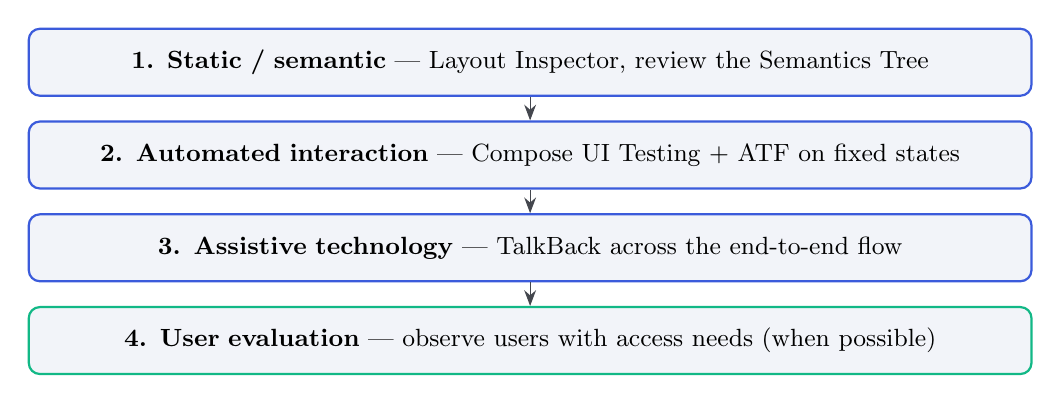
\begin{tikzpicture}[
  l/.style={rounded corners=4pt,draw,line width=0.8pt,minimum height=0.85cm,align=center,font=\small,text width=12.5cm,fill=softbg},
  e/.style={-{Stealth[length=2mm]},draw=slate}
]
  \node[l,draw=brandblue] (a) {\textbf{1. Static / semantic} --- Layout Inspector, review the Semantics Tree};
  \node[l,draw=brandblue,below=3mm of a] (b) {\textbf{2. Automated interaction} --- Compose UI Testing + ATF on fixed states};
  \node[l,draw=brandblue,below=3mm of b] (c) {\textbf{3. Assistive technology} --- TalkBack across the end-to-end flow};
  \node[l,draw=brandgreen,below=3mm of c] (d) {\textbf{4. User evaluation} --- observe users with access needs (when possible)};
  \draw[e] (a)--(b); \draw[e] (b)--(c); \draw[e] (c)--(d);
\end{tikzpicture}
\caption{The layered evaluation model. Each layer answers a different question; no single layer is
sufficient on its own.}
\label{fig:layers}
\end{figure}

\subsection{Manual testing with TalkBack}

TalkBack is the ground truth for the listening experience. Our protocol runs each core flow twice:
first swiping linearly to check focus order and labels, then exploring by touch to compare the visual
region with the focus region. For every important control we activate it and verify the role, state,
and \emph{post-action focus}. Common issues this surfaces --- and which pure automation misses ---
are wrong or missing labels, focus that jumps after a dialog, over-merged cards that hide a child
action, and dynamic changes (buffering, errors) that are never announced. We record each finding with
a severity, reproduction steps, and expected-vs-actual behaviour.

\subsection{Accessibility Scanner --- and an honest case study}

Accessibility Scanner evaluates a screen on-device and draws orange boxes around potential issues
(labels, touch targets, contrast). To practise the \emph{evidence-collection workflow} --- not to
judge another company's app --- we captured a 15-screen flow through Agoda
(Figure~\ref{fig:scanner}). The point of the exercise is methodological: how to record, de-duplicate,
and interpret tool output responsibly.

\begin{figure}[h]
\centering
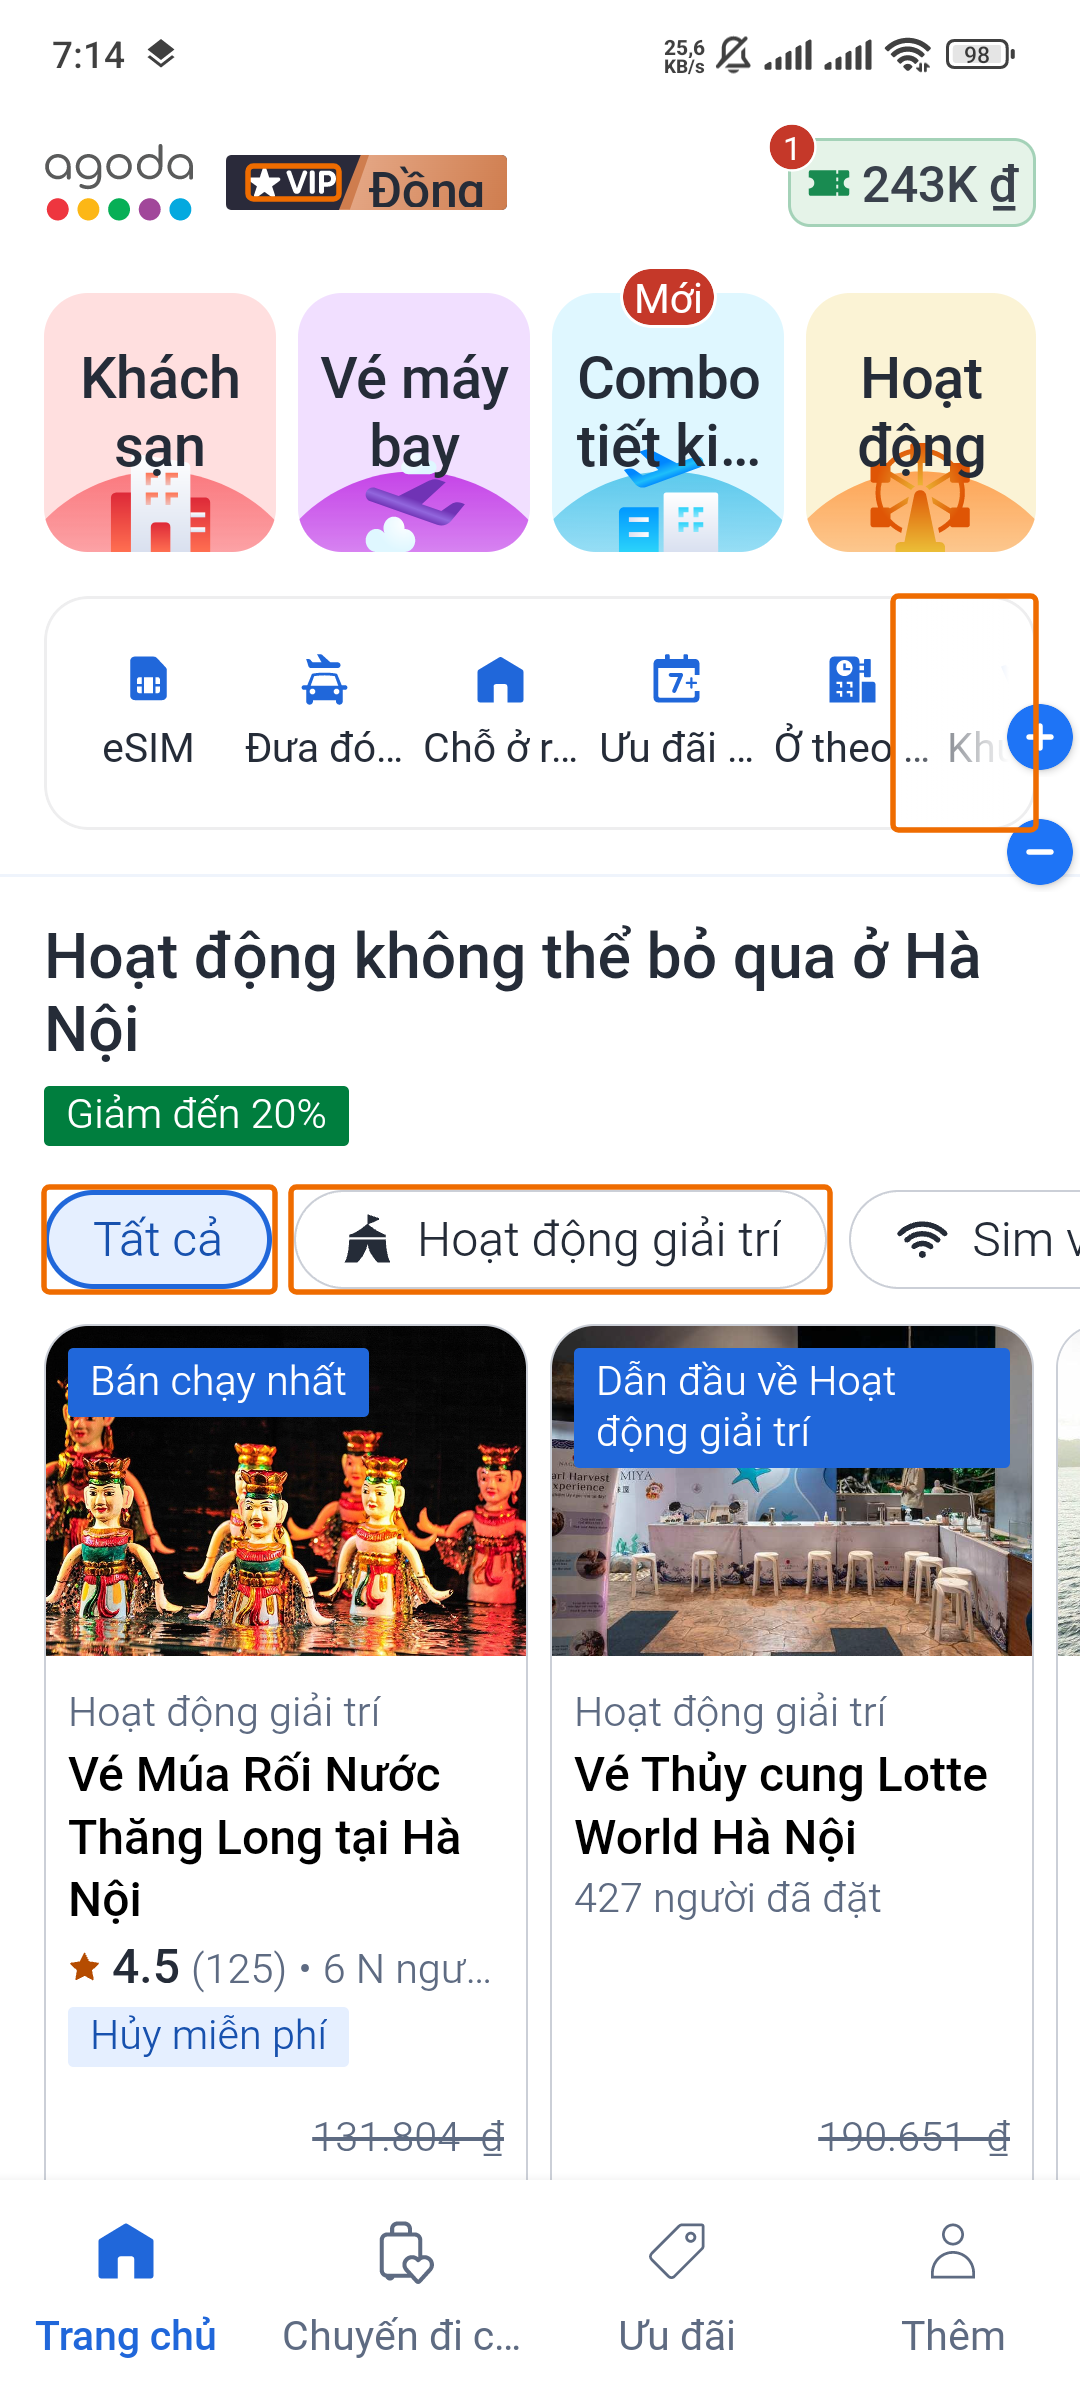
\includegraphics[height=8.6cm]{images/scanner_agoda.png}
\caption{Accessibility Scanner on a real app (Agoda), used only to rehearse the workflow. Orange
boxes mark raw \emph{suggestions} --- e.g. a 38\,dp touch target below the 48\,dp guideline and chips
that may lack a distinct label. Raw suggestions are not confirmed defects.}
\label{fig:scanner}
\end{figure}

The 15-screen capture produced \textbf{102 raw suggestions}, distributed as in
Figure~\ref{fig:dist}. These numbers must be read carefully: they are \emph{not} 102 independent,
confirmed bugs. Loading/skeleton states, web-view content, and the \emph{same} chip appearing across
several frames all inflate the count (report~2 and report~14 overlap; the splash screen produced
none). The correct next step is de-duplication by root cause and confirmation with TalkBack ---
never turning a warning into a conclusion without reproducing it.

\begin{figure}[h]
\centering
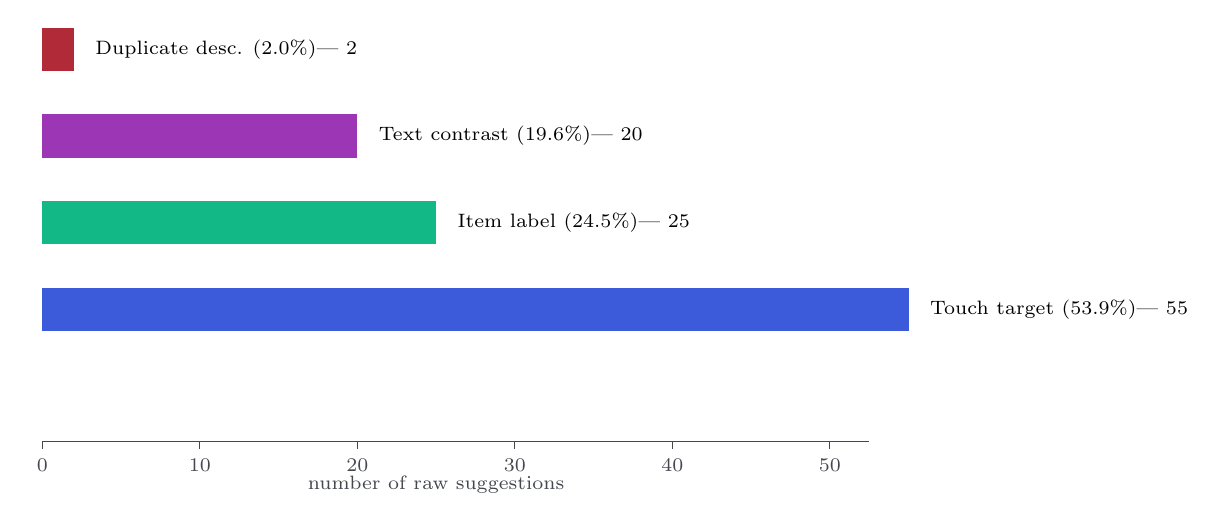
\begin{tikzpicture}
  \def\barh{0.55}
  % axis
  \draw[slate] (0,0) -- (10.5,0);
  \foreach \x/\lbl in {0/0,2/10,4/20,6/30,8/40,10/50} {
    \draw[slate] (\x,0)--(\x,-0.1) node[below,font=\scriptsize]{\lbl};
  }
  % bars: value scaled x/5
  \foreach \i/\val/\name/\col in {0/55/{Touch target (53.9\%)}/brandblue, 1/25/{Item label (24.5\%)}/brandgreen, 2/20/{Text contrast (19.6\%)}/codeann, 3/2/{Duplicate desc. (2.0\%)}/warnred} {
    \fill[\col] (0,{1.4+\i*(\barh+0.55)}) rectangle ({\val/5},{1.4+\i*(\barh+0.55)+\barh});
    \node[right,font=\scriptsize] at ({\val/5+0.15},{1.4+\i*(\barh+0.55)+\barh/2}) {\name --- \val};
  }
  \node[font=\scriptsize\color{slate}] at (5,-0.55) {number of raw suggestions};
\end{tikzpicture}
\caption{Distribution of the 102 raw suggestions across the 15-screen Agoda capture. Touch-target
warnings dominate, but this is a \emph{starting hypothesis}, not a root-cause finding.}
\label{fig:dist}
\end{figure}

\subsection{Layout Inspector, Compose UI Testing, and ATF}

Once we have our own source, three developer tools close the loop:

\begin{itemize}[leftmargin=1.4em]
  \item \textbf{Layout Inspector} shows the live merged and unmerged semantics trees, linking a
        TalkBack/Scanner symptom to a specific node --- a diagnostic tool, not a verdict on user
        experience.
  \item \textbf{Compose UI Testing} asserts semantics contracts in CI: that a control has the
        accessible name a screen reader will speak, and \code{printToLog()} dumps the tree for
        diagnosis. Our \code{AccessibilityTest.kt} does exactly this.
  \item \textbf{Accessibility Test Framework (ATF)}, Google's open-source rule engine, adds
        automated checks for speakable text, touch-target size, and contrast, usable as a CI quality
        gate.
\end{itemize}

\begin{lstlisting}[caption={\texttt{AccessibilityTest.kt} --- assert a spoken name, then dump the tree.},captionpos=b]
// 1. The icon-only search button must expose a spoken label, not just a glyph.
composeRule.onNodeWithContentDescription("Search podcasts").assertExists()

// 2. Dump the unmerged tree to verify merge/clear behaviour on the cards.
composeRule.onRoot(useUnmergedTree = true).printToLog("A11Y_TREE")
\end{lstlisting}

Table~\ref{tab:tools} positions each tool against the others.

\begin{table}[h]
\centering
\small
\begin{tabularx}{\textwidth}{@{}l l l Y@{}}
\toprule
\textbf{Tool} & \textbf{Source?} & \textbf{Mode} & \textbf{Best for / cannot replace} \\
\midrule
TalkBack & No & Manual & Listening experience, focus, end-to-end flow. \\
Accessibility Scanner & No & Semi-auto & Fast visual triage of labels/targets/contrast; not coverage. \\
Layout Inspector & Debug build & Manual & Inspect merged/unmerged tree; not user experience. \\
Compose UI Testing & Yes & Automated & Semantics contracts \& regression; not utterance quality. \\
ATF & Yes & Automated & Standardised checks in CI; not real usability. \\
\bottomrule
\end{tabularx}
\caption{Complementary roles of the five verification tools.}
\label{tab:tools}
\end{table}

\subsection{Evaluation metrics and trade-offs}

A credible evaluation states scope, representative flows, device, versions, and completion criteria,
then reports both automated and task-based measures: first-flow coverage, task-completion rate,
completion time, number of TalkBack gestures, automated pass rate, and a \emph{confirmed-defect
rate} that distinguishes real bugs from raw suggestions. Findings are triaged by \textbf{impact on
the task} --- \emph{Blocker} (task impossible, fix before ship) $>$ \emph{Major} $>$ \emph{Moderate}
$>$ \emph{Minor} --- not merely by count. A missing label on the checkout button outweighs many
touch-target warnings on secondary content.

Every technique in this report is a trade-off, and naming them is part of an honest evaluation:

\begin{itemize}[leftmargin=1.4em]
  \item \code{mergeDescendants} cuts swipes but can hide an independent child action or produce an
        over-long sentence --- measure gesture count \emph{and} listen to the whole utterance.
  \item Rich labels aid comprehension but, if they duplicate role/state, add listening time.
  \item \code{traversalIndex} fixes reading order but hand-tuned indices are brittle and can drift
        from the visual layout; use the minimum number and document why.
  \item Custom controls give design freedom but must re-declare role, state, and keyboard behaviour
        that Material would have provided for free.
\end{itemize}

\section{Conclusion}

Accessibility in Jetpack Compose is not a checkbox but a design discipline that spans the whole
stack. This project took an ordinary podcast UI and made it usable without sight by working the
semantics tree deliberately at every level: naming and hiding elements correctly
(Section~\ref{sec:core}), then shaping how those elements are grouped, ordered, and acted upon
(Section~\ref{sec:adv}). The result is a three-screen app in which a TalkBack user can discover a
show, choose an episode, and control playback --- hearing a clean sentence per card, reaching every
action through the actions menu, and getting spoken feedback the moment playback state changes.

Equally important is the evaluation discipline of Section~\ref{sec:test}: TalkBack answers the
listening question, Scanner triages quickly, Layout Inspector explains the structure, Compose UI
Testing protects semantics against regressions, and ATF automates the mechanical checks. The value
lies in \emph{combining} these layers, defining a clear scope, and --- as our Agoda case study
showed --- never mistaking a tool's raw suggestion for a confirmed defect.

Our broader takeaway is that accessible design is cheaper and better when it is built in from the
first composable rather than retrofitted: preferring Material components with sound default
semantics, reaching for custom semantics only where the design demands it, and testing with the same
assistive technology real users rely on. Building inclusively is, in the end, simply building well.

\subsection*{Future work}

The natural Version~2 is to run TalkBack on our own build across a device/version matrix, capture
Layout Inspector evidence for representative findings, expand the Compose test suite and wire ATF
into CI, and --- resources permitting --- invite users who rely on assistive technology to evaluate
the core tasks.

\section*{Appendix on AI usage}
\addcontentsline{toc}{section}{Appendix on AI usage}

AI assistants were used as a drafting and formatting aid: to help structure this report, generate the
LaTeX scaffolding and diagrams, and produce the annotated UI mockups from our own designs and code.
All accessibility techniques, the app architecture, the research decisions, and the case-study data
originate from the group's own work; every AI-assisted passage was reviewed and edited by the members
responsible for that section. Code samples in this report are excerpts from the app we wrote, not
AI-generated boilerplate.

\section{Appendix A --- Task division}
\addcontentsline{toc}{section}{Appendix A --- Task division}

\begin{table}[h]
\centering
\small
\begin{tabularx}{\textwidth}{@{}l l Y@{}}
\toprule
\textbf{Member} & \textbf{Research topic} & \textbf{Report \& demo responsibility} \\
\midrule
Phát   & Accessibility foundations & Introduction, Background: WCAG/POUR, EAA, TalkBack, Semantics vs Composition tree, \code{liveRegion} concept. \\
Phong  & Core Compose semantics & Technical Approach I: \code{contentDescription}, roles, \code{stateDescription}, 48\,dp targets, font scaling; fixed the app's basic UI defects. \\
Khương & Advanced semantics \& navigation & Technical Approach II: \code{mergeDescendants}, \code{clearAndSetSemantics}, \code{hideFromAccessibility}, \code{customActions}, traversal; built the advanced demos. \\
Tính   & Testing \& evaluation & Case-study integration, TalkBack/Scanner/Inspector/ATF testing, Evaluation, Conclusion; assembled the project and this report. \\
\bottomrule
\end{tabularx}
\caption{Division of research and writing across the group of four.}
\end{table}

\section{Appendix B --- Running the app}
\addcontentsline{toc}{section}{Appendix B --- Running the app}

\begin{enumerate}[leftmargin=1.4em]
  \item Open the \texttt{PodcastAccessibilityApp} folder in Android Studio (Koala or newer); let it
        sync and generate the Gradle wrapper and \texttt{local.properties}.
  \item Run the \texttt{app} configuration on an emulator or device (\texttt{minSdk 24},
        \texttt{targetSdk 34}).
  \item To experience the accessibility work, enable \textbf{TalkBack}, install
        \textbf{Accessibility Scanner}, and set the system \textbf{font size} to 200\%.
  \item Run the instrumented checks: \texttt{./gradlew connectedAndroidTest}.
\end{enumerate}

\textbf{Project layout.} \texttt{data/} holds the models and the \code{PodcastRepository} interface
with its mock; \texttt{ui/} holds the theme, navigation, and the \texttt{home}, \texttt{detail}, and
\texttt{player} screens. Section~\ref{sec:casestudy}, Table~\ref{tab:map} maps every technique to its
file.

\section*{Limitations of this report}
\addcontentsline{toc}{section}{Limitations}

This is a front-end study. The app ships with mocked data and no real audio engine, so performance
and networked-state accessibility (e.g. announcing buffering under poor connectivity) are described
at the design level rather than measured. The Agoda case study used a single device and one capture
pass; its figures demonstrate the evidence-collection \emph{process} and must not be read as an audit
of Agoda. Absolute WCAG conformance is likewise not claimed --- only a principled mapping of
technology-neutral criteria onto Android.


\clearpage
\begin{thebibliography}{99}
\addcontentsline{toc}{section}{References}

\bibitem{a11y-principles} Android Developers.
\emph{Principles for improving app accessibility}. developer.android.com. Accessed 22 Jul 2026.

\bibitem{compose-semantics} Android Developers.
\emph{Semantics in Compose}. developer.android.com/develop/ui/compose/semantics.

\bibitem{talkback} Google.
\emph{Get started on Android with TalkBack}. Android Accessibility Help.

\bibitem{merging} Android Developers.
\emph{Merging and clearing (Jetpack Compose accessibility)}. developer.android.com.

\bibitem{scanner} Google.
\emph{Accessibility Scanner}. Google Play / Android Accessibility Help.

\bibitem{scanner-video} Android Developers.
\emph{Accessibility Scanner --- Accessibility on Android} (video).

\bibitem{layout-inspector} Android Developers.
\emph{Debug your layout with Layout Inspector} (Compose semantics view).

\bibitem{semantics-guide} Android Developers.
\emph{Accessibility in Compose --- key concepts and the semantics tree}.

\bibitem{unmerged} Android Developers.
\emph{Test your Compose layout --- merged and unmerged semantics trees}.

\bibitem{traversal} Android Developers.
\emph{Modify traversal order} (\code{isTraversalGroup}, \code{traversalIndex}).

\bibitem{compose-testing} Android Developers.
\emph{Testing your Compose layout --- semantics matchers, assertions, printToLog}.

\bibitem{atf-compose} Android Developers.
\emph{Automated accessibility checks in Compose tests} (ATF integration, Compose 1.8+).

\bibitem{atf} Google.
\emph{Accessibility Test Framework for Android} (open-source repository).

\bibitem{espresso-a11y} Android Developers.
\emph{Accessibility checking with Espresso} (\code{AccessibilityChecks.enable()}).

\bibitem{w3c-tools} W3C Web Accessibility Initiative (WAI).
\emph{Selecting Web Accessibility Evaluation Tools} --- automation covers only part of conformance.

\bibitem{wcag22} W3C.
\emph{Web Content Accessibility Guidelines (WCAG) 2.2}. W3C Recommendation, 2023.

\bibitem{wcag2ict} W3C.
\emph{WCAG2ICT --- Applying WCAG to Non-Web Information and Communications Technologies}.

\bibitem{wcag-em} W3C WAI.
\emph{Website Accessibility Conformance Evaluation Methodology (WCAG-EM) 1.0}.

\bibitem{involving-users} W3C WAI.
\emph{Involving Users in Evaluating Web Accessibility}.

\bibitem{iso9241} ISO.
\emph{ISO 9241-11:2018 --- Usability: definitions and concepts} (effectiveness, efficiency,
satisfaction).

\bibitem{mobile-a11y} W3C WAI.
\emph{Mobile Accessibility: How WCAG 2 and other WAI guidelines apply to mobile}.

\bibitem{material-a11y} Google.
\emph{Material Design --- Accessibility} (touch targets, contrast).

\bibitem{eaa} European Commission.
\emph{European Accessibility Act (Directive (EU) 2019/882)}.

\bibitem{font-scaling} Android Developers.
\emph{Android 14 features --- non-linear font scaling}.

\bibitem{appt-actions} Appt.org.
\emph{Accessibility action in Jetpack Compose}.

\end{thebibliography}


\end{document}
